\chapter{Experimental Result} % Main chapter title

\label{Chapter 6} 
\lhead{Chapter 6. \emph{Experimental Result}} 

In this chapter, we would discuss various result.

\section{Global Histogram using only magnitudes of optical flow}
In this section, we would discuss the experimental result for Global Histogram using only magnitudes of optical flow. Since we have used only the magnitude part, there is poor accuracy.
There is a lot of information loss through orientation flow part.

\begin{table}[]
\centering
\hspace*{-2.5cm}
\begin{tabular}{|l|l|l|l|l|l|l|l|l|l|}
\hline
\textbf{Evaluation} &
  \multicolumn{3}{c|}{\textbf{Accuracy}} &
  \multicolumn{2}{c|}{\textbf{Precision}} &
  \multicolumn{2}{c|}{\textbf{Recall}} &
  \multicolumn{2}{c|}{\textbf{F1}} \\ \hline
Adavus         & MF + KF & MF    & KF    & MF    & KF    & MF    & KF    & MF    & KF    \\ \hline
Tatta          & 52.1    & 66.48 & 45.78 & 35.01 & 75.66 & 66.48 & 45.78 & 45.86 & 57.04 \\ \hline
Natta          & 59.26   & 64.3  & 55.32 & 52.92 & 66.49 & 64.3  & 55.32 & 58.06 & 60.39 \\ \hline
Kuditta Mettu  & 71.07   & 62.24 & 77.19 & 65.45 & 74.66 & 62.24 & 77.19 & 63.81 & 75.9  \\ \hline
Kuditta Nattal & 67.73   & 62.67 & 74.47 & 76.54 & 60.01 & 62.67 & 74.47 & 68.91 & 66.46 \\ \hline
Kuditta Tattal & 54.72   & 44.95 & 69.16 & 68.3  & 45.93 & 44.95 & 69.16 & 54.22 & 55.2  \\ \hline
Tei Tei Dhatta & 54.19   & 45.51 & 77.69 & 84.66 & 34.51 & 45.51 & 77.69 & 59.2  & 47.79 \\ \hline
Katti Kartari  & 68.88   & 63.04 & 80    & 85.71 & 53.2  & 63.04 & 80    & 72.65 & 63.91 \\ \hline
Utsanga        & 45.79   & 37.04 & 67.27 & 73.53 & 30.33 & 37.04 & 67.27 & 49.26 & 41.81 \\ \hline
Mandi          & 72.75   & 67.04 & 78.98 & 77.67 & 68.72 & 67.04 & 78.98 & 71.97 & 73.49 \\ \hline
Tirmana        & 48.51   & 35.45 & 69.82 & 65.71 & 39.87 & 35.45 & 69.82 & 46.06 & 50.75 \\ \hline
Sarika         & 47.81   & 33.91 & 70.39 & 65.06 & 39.58 & 33.91 & 70.39 & 44.59 & 50.67 \\ \hline
Joining        & 65.79   & 62.11 & 71    & 75.16 & 57.01 & 62.11 & 71    & 68.01 & 63.25 \\ \hline
\end{tabular}
\caption{Used only magnitudes for binning}
\label{tab:Ch06T001}
\end{table}


\begin{figure}[H]
    \hspace{-2.5cm}
    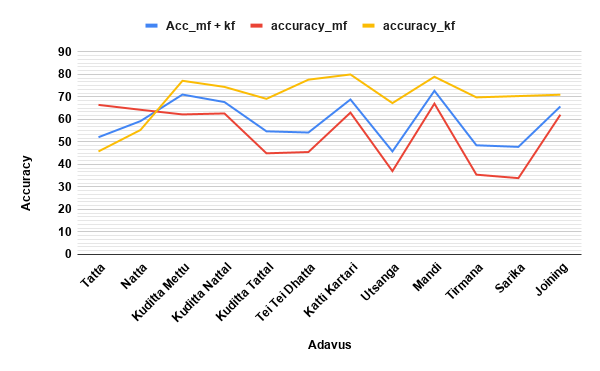
\includegraphics[scale= 0.8]{./Pictures/hist.png}
    \caption{Testing Module}
    \label{fig:Ch06F001}
\end{figure}

From the plot, we can see that accuracy for Keyframe is always higher than the accuracy of the motion frame except for two cases of Tatta and Natta.
Accuracy for motion frame and Keyframe combined lies between accuracy for Keyframe and motion frame except for two cases of Tatta and Natta. It is mainly due to the simple motion frame structure as compared to Keyframe in Tattaand Natta.



\section{Global Histogram using  magnitudes and Orientation of optical flow}
In this section, we would discuss the experimental result for global Histogram using magnitudes and orientation of optical flow since we have used the magnitude and orientation of optical flow. There should be better accuracy than better accuracy.
We have more information from the orientation of optical flow


\begin{table}[]
\centering
\hspace*{-1cm}
\begin{tabular}{|l|l|l|l|l|l|l|l|l|l|}
\hline
\multicolumn{1}{|c|}{\textbf{Evaluation}} &
  \multicolumn{3}{c|}{\textbf{Accuracy}} &
  \multicolumn{2}{c|}{\textbf{Precision}} &
  \multicolumn{2}{c|}{\textbf{Recall}} &
  \multicolumn{1}{c|}{\textbf{F1}} &
  \multicolumn{1}{c|}{\textbf{F1}} \\ \hline
\multicolumn{1}{|c|}{\textbf{Adavus}} &
  \multicolumn{1}{c|}{\textbf{MF + KF}} &
  \multicolumn{1}{c|}{\textbf{MF}} &
  \multicolumn{1}{c|}{\textbf{KF}} &
  \multicolumn{1}{c|}{\textbf{MF}} &
  \multicolumn{1}{c|}{\textbf{KF}} &
  \multicolumn{1}{c|}{\textbf{MF}} &
  \multicolumn{1}{c|}{\textbf{KF}} &
  \multicolumn{1}{c|}{\textbf{MF}} &
  \multicolumn{1}{c|}{\textbf{KF}} \\ \hline
Tatta          & 73.07 & 64.38 & 76.89 & 55.04 & 83.09 & 64.38 & 76.89 & 59.34 & 79.87 \\ \hline
Natta          & 73.79 & 67.28 & 78.88 & 71.33 & 75.53 & 67.28 & 78.88 & 69.25 & 77.17 \\ \hline
Kuditta Mettu  & 82.72 & 74.41 & 88.49 & 81.77 & 83.28 & 74.41 & 88.49 & 77.92 & 85.81 \\ \hline
Kuditta Nattal & 76.73 & 72.3  & 82.61 & 84.68 & 69.18 & 72.3  & 82.61 & 78    & 75.3  \\ \hline
Kuditta Tattal & 67.55 & 60.2  & 78.42 & 80.49 & 57.13 & 60.2  & 78.42 & 68.88 & 66.1  \\ \hline
Tei Tei Dhatta & 64.09 & 57.88 & 80.88 & 89.12 & 41.51 & 57.88 & 80.88 & 70.18 & 54.86 \\ \hline
Katti Kartari  & 70.66 & 64.59 & 82.22 & 87.37 & 54.95 & 64.59 & 82.22 & 74.27 & 65.88 \\ \hline
Utsanga        & 59.47 & 57.04 & 65.45 & 80.21 & 38.3  & 57.04 & 65.45 & 66.67 & 48.32 \\ \hline
Mandi          & 80.05 & 76.17 & 84.29 & 84.1  & 76.43 & 76.17 & 84.29 & 79.94 & 80.17 \\ \hline
Tirmana        & 61.21 & 53.53 & 73.73 & 76.88 & 49.31 & 53.53 & 73.73 & 63.11 & 59.1  \\ \hline
Sarika         & 51.18 & 35.55 & 76.6  & 71.18 & 42.23 & 35.55 & 76.6  & 47.42 & 54.44 \\ \hline
Joining        & 71.49 & 68.68 & 75.46 & 79.82 & 63.04 & 68.68 & 75.46 & 73.83 & 68.7  \\ \hline
\end{tabular}
\caption{Used magnitudes and Orientation for binning}
\label{tab:Ch06T002}
\end{table}








\begin{figure}[H]
    \hspace{-2.5cm}
    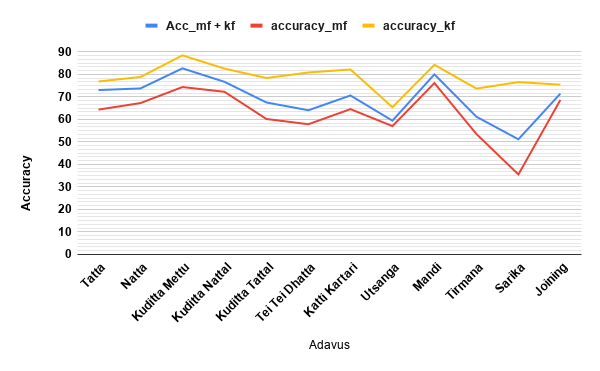
\includegraphics[scale= 0.8]{./Pictures/global.png}
    \caption{Testing Module}
    \label{fig:Ch06F002}
\end{figure}


\section{Fractional Histogram Binning using  magnitudes and Orientation of optical flow taken over 8 x 8 cell}



\begin{table}[]
\hspace*{-1.25cm}
\begin{tabular}{|l|l|l|l|l|l|l|l|l|l|}
\hline
Evaluation & \multicolumn{3}{l|}{Accuracy} & \multicolumn{2}{l|}{Precision} & \multicolumn{2}{l|}{Recall} & F1 & F1 \\ \hline
Adavus         & MF + KF & MF    & KF    & MF    & KF    & MF    & KF    & MF    & KF    \\ \hline
Tatta          & 87.76   & 73.63 & 93.96 & 84.27 & 89.03 & 73.63 & 93.96 & 78.59 & 91.43 \\ \hline
Natta          & 79.83   & 71.75 & 86.14 & 80.17 & 79.61 & 71.75 & 86.14 & 75.73 & 82.75 \\ \hline
Kuditta Mettu  & 81.04   & 69.98 & 88.71 & 81.14 & 80.98 & 69.98 & 88.71 & 75.15 & 84.67 \\ \hline
Kuditta Nattal & 77.2    & 82.61 & 70.15 & 78.29 & 75.59 & 82.61 & 70.15 & 80.39 & 72.77 \\ \hline
Kuditta Tattal & 77.5    & 70.2  & 88.42 & 90.49 & 67.13 & 70.2  & 88.42 & 78.88 & 76.1  \\ \hline
Tei Tei Dhatta & 81.08   & 88.66 & 60.56 & 85.88 & 66.38 & 88.66 & 60.56 & 87.25 & 63.33 \\ \hline
Katti Kartari  & 82.65   & 88.33 & 71.85 & 85.66 & 76.38 & 88.33 & 71.85 & 86.97 & 74.05 \\ \hline
Utsanga        & 78.95   & 85.19 & 63.64 & 85.19 & 63.64 & 85.19 & 63.64 & 85.19 & 63.64 \\ \hline
Mandi          & 80.59   & 85.26 & 73.98 & 82.23 & 78.04 & 85.26 & 73.98 & 83.72 & 75.95 \\ \hline
Tirmana        & 77.39   & 82.37 & 69.06 & 81.66 & 70.07 & 82.37 & 69.06 & 82.01 & 69.57 \\ \hline
Sarika         & 70.36   & 69.9  & 71.1  & 79.73 & 59.23 & 69.9  & 71.1  & 74.49 & 64.63 \\ \hline
Joining        & 80.59   & 85.26 & 73.98 & 82.23 & 78.04 & 85.26 & 73.98 & 83.72 & 75.95 \\ \hline
\end{tabular}
\caption{result: fractional histogram binning}
\label{tab:Ch06T003}
\end{table}



















\begin{figure}[H]
    % \centering
    \hspace{-2.5cm}
    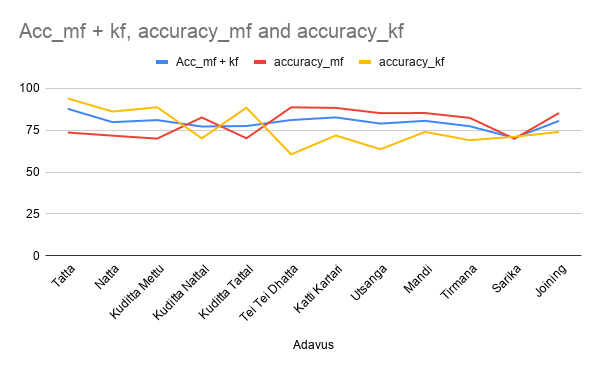
\includegraphics[scale= 0.8]{./Pictures/local.png}
    \caption{Testing Module}
    \label{fig:Ch06F003}
\end{figure}





\section{Comparison among different histogram approaches}






\begin{table}[]
\hspace{-2.5cm}
\begin{tabular}{|c|c|c|c|c|c|c|}
\hline
Approach       & Approach 1 & Approach 2 & Approach 3 & Approach 1 & Approach 2 & Approach 3 \\ \hline
Adavus         & \multicolumn{3}{c|}{MF}              & \multicolumn{3}{c|}{KF}              \\ \hline
Tatta          & 66.48      & 64.38      & 73.63      & 45.78      & 76.89      & 93.96      \\ \hline
Natta          & 64.30      & 67.28      & 71.75      & 55.32      & 78.88      & 86.14      \\ \hline
Kuditta Mettu  & 62.24      & 74.41      & 69.98      & 77.19      & 88.49      & 88.71      \\ \hline
Kuditta Nattal & 62.67      & 72.30      & 82.61      & 74.47      & 82.61      & 70.15      \\ \hline
Kuditta Tattal & 44.95      & 60.20      & 70.20      & 69.16      & 78.42      & 88.42      \\ \hline
Tei Tei Dhatta & 45.51      & 57.88      & 88.66      & 77.69      & 80.88      & 60.56      \\ \hline
Katti Kartari  & 63.04      & 64.59      & 88.33      & 80.00      & 82.22      & 71.85      \\ \hline
Utsanga        & 37.04      & 57.04      & 85.19      & 67.27      & 65.45      & 63.64      \\ \hline
Mandi          & 67.04      & 76.17      & 85.26      & 78.98      & 84.29      & 73.98      \\ \hline
Tirmana        & 35.45      & 53.53      & 82.37      & 69.82      & 73.73      & 69.06      \\ \hline
Sarika         & 33.91      & 35.55      & 69.90      & 70.39      & 76.60      & 71.10      \\ \hline
Joining        & 62.11      & 68.68      & 85.26      & 71.00      & 75.46      & 73.98      \\ \hline
\end{tabular}
\caption{Comparision between various approaches}
\label{tab:Ch06T004}
\end{table}











\begin{figure}[H]
    % \centering
    \hspace{-2.5cm}
    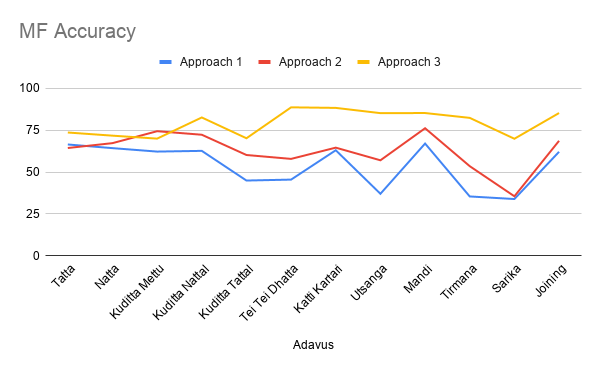
\includegraphics[scale= 0.8]{./Pictures/mf.png}
    \caption{Testing Module}
    \label{fig:Ch06F004}
\end{figure}

\begin{figure}[H]
    % \centering
    \hspace{-2.5cm}
    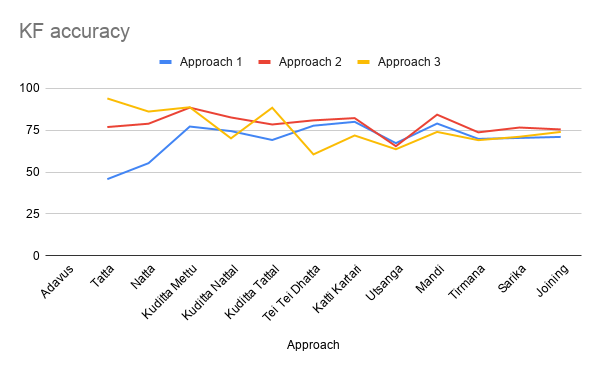
\includegraphics[scale= 0.8]{./Pictures/kf.png}
    \caption{Testing Module}
    \label{fig:Ch06F005}
\end{figure}





\section{Minimum accuracy plot}
    % \centering
    \begin{figure}[H]
    \hspace{-2.5cm}    
    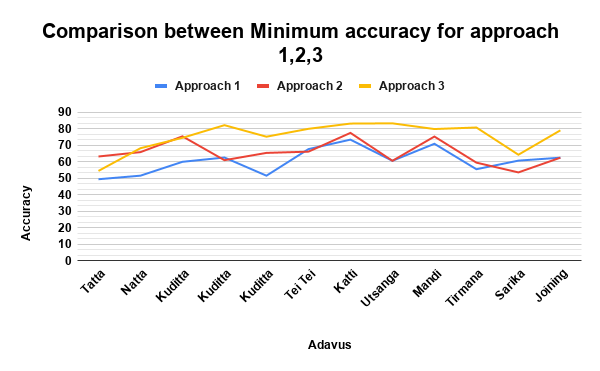
\includegraphics[scale= 0.8]{./Pictures/min.png}
    \caption{Minimum accuracy plot}
    \label{fig:Ch06F006}
\end{figure}

\section{Maximum accuracy plot}
    % \centering
    \begin{figure}[H]
    \hspace{-2.5cm}
    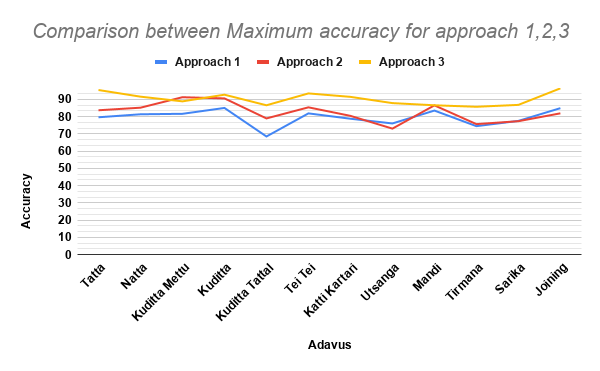
\includegraphics[scale= 0.8]{./Pictures/max.png}
    \caption{Maximum accuracy plot}
    \label{fig:Ch06F007}
\end{figure}
